\subsection{Lighting}
\label{sec:lighting}

\textbf{Purpose}: Discrete light spectrum and intensity control to provide all light necessary for plant growth, as well as sanitization.

\textbf{Function}:
\begin{itemize}
    \item \textbf{Inputs}: Power, lighting spectrum-intensity control signal (aka per-LED modulation signals)
    \item \textbf{Outputs}: Light
\end{itemize}

\textbf{Method}:
\begin{enumerate}
    \item \textit{Setup}:
    \begin{enumerate}
        \item Connect power and spectrum-intensity control signal to driver board;
        \item Mount driver board and many LED boards to lighting tray;
        \item Daisy-chain LED boards, connect first and last to driver board;
    \end{enumerate}
    \item \textit{Testing}:
    \begin{itemize}
        \item Spectrum-intensity distribution control signal modulates LED power as expected;
        \item Passive heat sinks dissipate enough heat;
    \end{itemize}
    \item \textit{Process}:
    \begin{enumerate}
        \item Power is delivered to drivers;
        \item Control signals "dim" drivers to modulate intensity distribution across spectrum;
        \item Power drivers power LEDs (one per wavelength/"series");
        \item LEDs emit light;
    \end{enumerate}
    \item \textit{Shutdown}:
    \begin{enumerate}
        \item Disconnect power and signals;
        \item Disconnect and dismount boards;
    \end{enumerate}
\end{enumerate}

\textbf{Features}:
\begin{itemize}
    \item \textit{LED Lights}: LEDs offer high power output, better efficiency and thermal management, lower footprint, and precise wavelengths while minimizing risk of damaging plant tissues. Many discretely-controlled wavelength options/"series" enable wide and fine control of intensity-spectrum distribution, with a focus on Photosynthetically-Active Radiation (PAR), as well as sanitization wavelengths and wavelengths to induce specific phenotypic and chemical changes. Located across multiple smaller daisy-chained PCBs to minimize cost. LED series include:
    \begin{itemize}
        \item Ultraviolet (267nm\footnote{This is the ideal wavelength for targeting a variety of pathogens, notably \textit{E. coli} \cite{uvecoli}}) \cite{led_uv};
        \item Blue (448nm) \cite{led_xpg3};
        \item Cool White (5700K) \cite{led_xpg3};
        \item Warm White (2700K) \cite{led_xpg3};
        \item Red (645nm) \cite{led_xpg3};
        \item Near-Infrared (730nm) \cite{led_xpe2};
    \end{itemize}
    \item \textit{LED Power Drivers}: High-efficiency constant-current PWM-dimmable DC-DC buck converters, specialized for LEDs \cite{leddriver}. One per series, driving a set of identical LEDs. One driver per lighting tray.
    % \item \textit{Heat Sink}: Passive cooling solution for LEDs. Mounted to opposing face of PCB.
\end{itemize}

\clearpage

\textbf{Figures}

\begin{figure}[h!]
    \centering
    \begin{subfigure}{.34\textwidth}
        \centering
        \frame{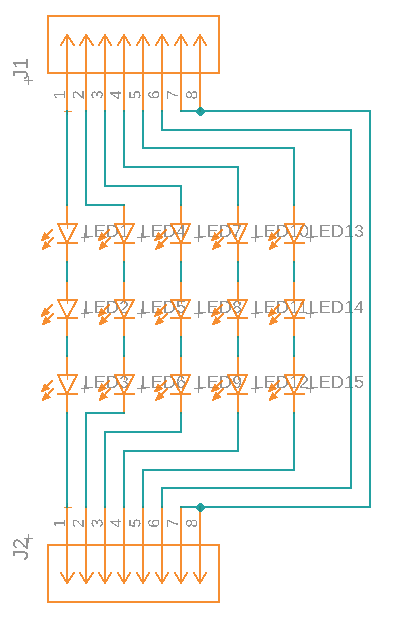
\includegraphics[width=\textwidth]{../assets/schematics/lighting_led_sch.png}}
        \caption{Schematic.}
        \label{fig:lighting_led_sch}
      \end{subfigure}
      \hspace{.08\textwidth}
      \begin{subfigure}{.35\textwidth}
        \centering
        \frame{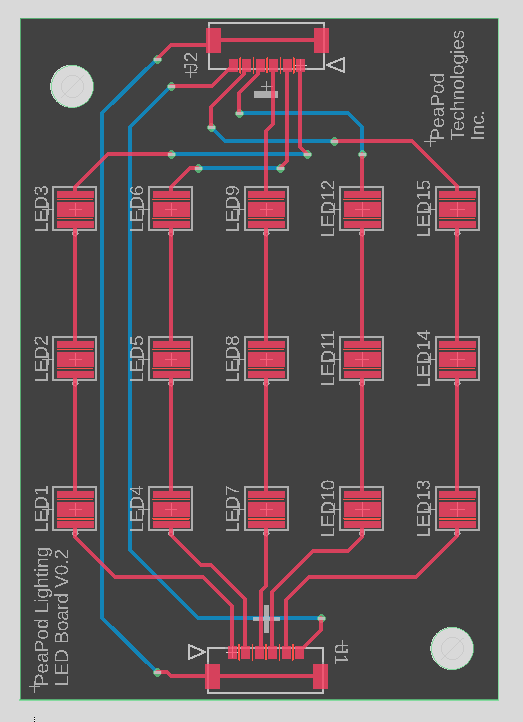
\includegraphics[width=\textwidth]{../assets/schematics/lighting_led_brd.png}}
        \caption{PCB layout.}
        \label{fig:lighting_led_brd}
      \end{subfigure}
      \caption{Lighting LED board.}
\end{figure}

\begin{figure}[h!]
    \centering
    \begin{subfigure}{.35\textwidth}
        \centering
        \frame{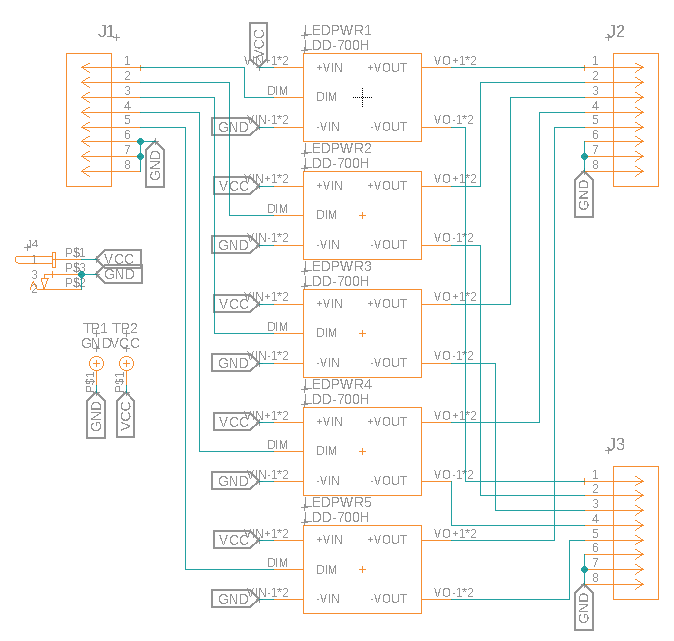
\includegraphics[width=\textwidth]{../assets/schematics/lighting_power_sch.png}}
        \caption{Schematic.}
        \label{fig:lighting_power_sch}
      \end{subfigure}
      \hspace{.02\textwidth}
      \begin{subfigure}{.6\textwidth}
        \centering
        \frame{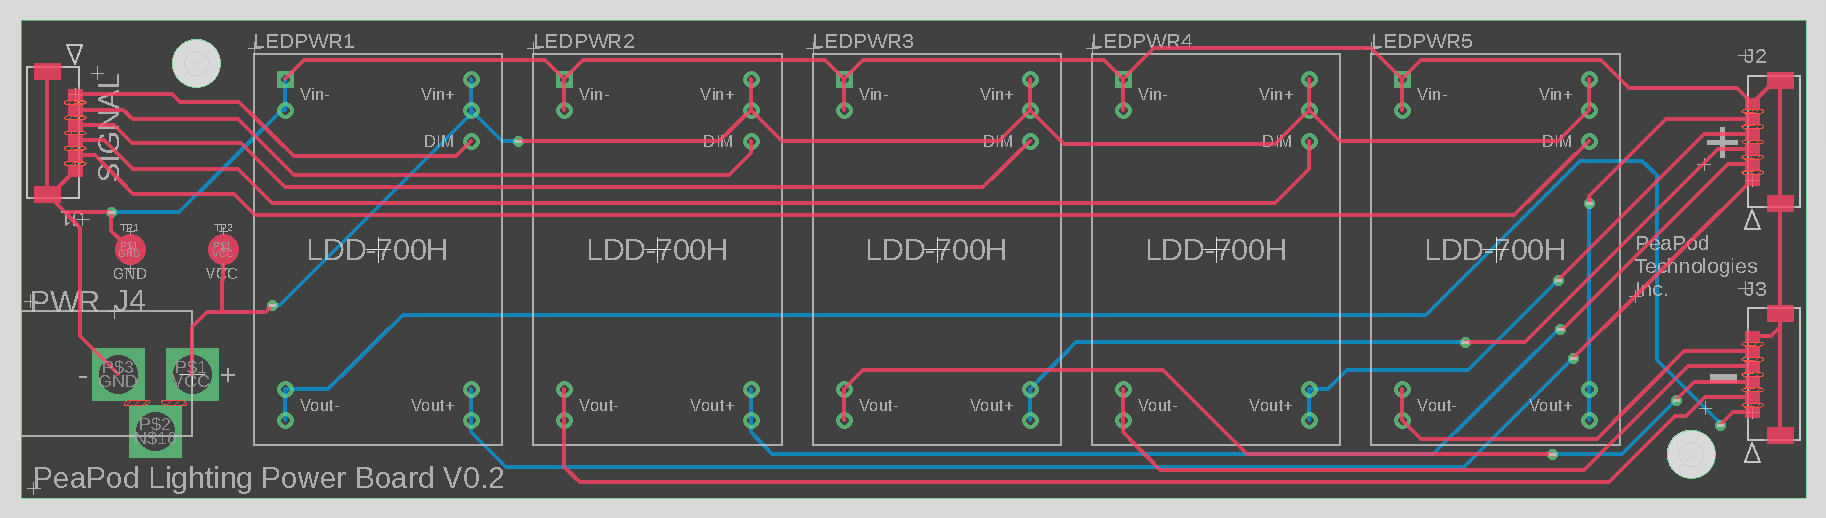
\includegraphics[width=\textwidth]{../assets/schematics/lighting_power_brd.png}}
        \caption{PCB layout.}
        \label{fig:lighting_power_brd}
      \end{subfigure}
      \caption{Lighting power board.}
\end{figure}